\documentclass[11pt,reqno]{amsart}
\usepackage[T1]{fontenc}
\usepackage{lmodern}
\usepackage[a4paper,textwidth=155mm,textheight=244mm,centering,headsep=6mm,footskip=10mm]{geometry}
\usepackage{microtype,mathtools,booktabs}
\usepackage{tikz,flafter}
\usepackage[hidelinks]{hyperref}
\numberwithin{equation}{section}
\newtheorem{theorem}{Theorem}[section]
\newtheorem{lemma}[theorem]{Lemma}
\newtheorem{proposition}[theorem]{Proposition}
\newtheorem{corollary}[theorem]{Corollary}
\newcommand{\Z}{\mathbb Z}
\setlength{\emergencystretch}{1.2em}
\title[The unfair 0--1 conjecture for trinomial factors]{The unfair 0--1 polynomial conjecture\\ for trinomial factors}
\date{18 November 2026}
\hypersetup{pdftitle={The unfair 0-1 polynomial conjecture for trinomial factors}}
\begin{document}
\begin{abstract}
Let two monic polynomials with nonnegative real coefficients have a product whose coefficients are all zero or one. If one factor has exactly three nonzero terms, we prove that every nonzero coefficient in both factors equals one. The exponents of the three terms and the degree of the other factor are arbitrary. Equivalently, if two independent, finitely supported integer-valued random variables have a sum uniform on its support, and one takes exactly three values, each is uniform on its own support. A fractional middle coefficient would have an algebraic conjugate of modulus greater than one. At this conjugate the recurrence forces certain differences between coefficients of the other factor to grow. We bound explicit linear combinations of these differences by counting walks on the integers and applying polynomial approximation on a real interval.
\end{abstract}
\maketitle

\section{Statement and normalization}
Call a polynomial \emph{binary} if all its coefficients are zero or one. A monic polynomial has leading coefficient one. A binary polynomial is \emph{fair} if, in every factorization into monic polynomials with nonnegative real coefficients, both factors are binary. The unfair 0--1 polynomial conjecture asserts that every monic binary polynomial is fair. We prove the conjectured conclusion whenever one factor has three nonzero terms.
\begin{theorem}\label{thm:main}
Let $A,B\in\mathbb R[X]$ be monic with nonnegative coefficients. If $AB$ is binary and $A$ has exactly three nonzero terms, then $A$ and $B$ are binary.
\end{theorem}
Ghidelli proved the case of exponents $0,2,5$ by studying a recurrence for the cofactor~\cite{ghidelli}. For exponents $0,2,m$, Dvorsky's combined theorem covers $m\ge7$~\cite[Theorem~1.1]{dvorsky}, using a companion manuscript for odd $7\le m\le339$~\cite{dvorsky-finite}. Hare tested patterns of zero, one, and fractional coefficients in candidate factors of degree at most fifteen~\cite{hare}. Hasanbegovi\'c gave a sufficient separation between two blocks of product coefficients for fairness of the lower block to imply fairness of the whole product~\cite{hasanbegovic}.

For the probabilistic formulation, translate both supports to start at zero. By independence, the probability generating polynomials multiply to that of the sum. If the sum is uniform on its support, dividing each factor by its leading coefficient makes the product binary. Theorem~\ref{thm:main} then gives uniformity on each support.

Conversely, given $A,B$ as in the theorem, take independent variables with generating polynomials $A/A(1)$ and $B/B(1)$. Their sum has generating polynomial $AB/(A(1)B(1))$, so its law is uniform on its support. The probabilistic assertion makes the positive coefficients of $A$ equal, and likewise for $B$. Monicity makes their common value one in each factor.

Remove the largest power of $X$ dividing each factor. The resulting constant terms are positive and multiply to one. Each is at most one, since it contributes to a coefficient of the product with the opposite leading coefficient. Hence both constant terms equal one. Pairing with the opposite constant term now bounds every coefficient by one. Write
\[
 A=1+aX^r+X^m,\qquad B=\sum_n b_nX^n,\qquad C=AB=\sum_n c_nX^n
\]
with $0<r<m$ and $0<a\le1$. Set coefficients outside the respective supports to zero. The basic equation is
\begin{equation}\label{eq:basic}
 b_n+b_{n-m}+a b_{n-r}=c_n\in\{0,1\}.
\end{equation}
If $a=1$, induction on $n$ gives $b_n\in\Z$ and hence $b_n\in\{0,1\}$. Suppose $0<a<1$. When $m=2r$, equation~\eqref{eq:basic} gives $b_r=1-a$ and $c_{2r}\ge1+a(1-a)>1$. In the other cases we may reverse both polynomials, replacing each $P(X)$ by $X^{\deg P}P(1/X)$, so that $m>2r$.

\begin{lemma}\label{lem:annulus}
The middle coefficient $a$ has an algebraic conjugate $\lambda$ of modulus $1<|\lambda|\le2$.
\end{lemma}
\begin{proof}
Every root of $A$ is a root of the monic integer polynomial $C$ and hence an algebraic integer. The coefficients of $A$ are signed elementary symmetric functions of those roots, so $a$ is an algebraic integer. Its conjugates, the roots of its minimal polynomial over $\mathbb Q$, have product a nonzero integer up to sign. Since $0<a<1$, one conjugate $\lambda$ has modulus greater than one.

By~\eqref{eq:basic}, every $b_n$ belongs to $\Z[a]$. Let $\sigma:\mathbb Q(a)\to\mathbb C$ take $a$ to $\lambda$. The finite set of values $\sigma(b_n)$ contains zero and one. If $b_n>0$, the digit $c_{n+r}$ is one, so
\[
 1-\lambda\sigma(b_n)=\sigma(b_{n+r})+\sigma(b_{n+r-m}).
\]
For $b_n=0$ the left side is $1=1+0$. Thus for every value $z$ in the set, $1-\lambda z$ is the sum of two values in it. Choose two points at the greatest distance $d$. Subtracting their two sums gives $|\lambda|d\le2d$ by the triangle inequality, and $d\ge1$.
\end{proof}
Fix such an embedding and put $R=|\lambda|$. We use the recurrence twice. At $a$, nonnegativity forces a stretch of at least five consecutive steps on which four neighboring equations all have right-hand side one. At $\lambda$, these ones survive the embedding. Subtracting successive equations along the stretch cancels their right-hand sides and forces growth in the cofactor differences. Taking a longest such stretch bounds the initial values inherited from its predecessor. Sections~\ref{sec:filter} and~\ref{sec:short} compare this growth with an upper bound on the same linear combinations of differences. The upper bound uses only the binary digits of the full product and is independent of its degree.

\section{The lowest positive coefficient in each column}\label{sec:bottom}
Place $b_{im+\ell r}$ in row $i$, column $\ell$, and denote it by $b_{i,\ell}$. Make the same array for the product digits $c_{i,\ell}$. For example, for $r=2$, $m=5$ the entries of row zero starting at column zero are $b_0,b_2,b_4,\ldots$, and the row immediately above starts $b_5,b_7,b_9,\ldots$. A step right adds $r$ to the exponent and a step up adds $m$. Thus
\begin{equation}\label{eq:array}
 b_{i,\ell}+b_{i-1,\ell}+a b_{i,\ell-1}=c_{i,\ell}.
\end{equation}
The array may repeat coefficients or use only indices divisible by $\gcd(r,m)$. Every displayed equation still follows from~\eqref{eq:basic}.

\begin{lemma}\label{lem:geometry}
Every column has a lowest positive entry. Its row $s(\ell)$ satisfies
\[
 s(\ell)\le s(\ell-1),\qquad s(\ell+m)=s(\ell)-r .
\]
Call a strict decrease a \emph{drop}. If its depth is $d=s(\ell-1)-s(\ell)$, the $d$ entries from the new bottom up to just below the old bottom are binary. They start with one, end with zero, and have no adjacent ones. Over one period, the depths of the drops sum to $r$ and the distances between consecutive drops sum to $m$.
\end{lemma}
\begin{proof}
Suppose $b_{i,\ell-1}>0$. Then $0<a b_{i,\ell-1}<1$. Equation~\eqref{eq:array} forces $c_{i,\ell}=1$ and
\[
 b_{i,\ell}+b_{i-1,\ell}=1-a b_{i,\ell-1}>0.
\]
Thus the next column has a positive entry at or below row $i$. Starting with $b_{0,0}=1$ gives nonempty columns to the right. The identity $b_{i,\ell+m}=b_{i+r,\ell}$ gives nonemptiness for all integer $\ell$. Each column has finite support, so its bottom exists. Taking $i=s(\ell-1)$ proves monotonicity, and the same shift identity gives the formula for $s(\ell+m)$.

At a drop write $s=s(\ell)$ and $p=s(\ell-1)$. In rows $s\le i<p$ the left neighbor is zero, so $b_{i,\ell}+b_{i-1,\ell}$ is a binary digit. The entry below $s$ is zero and the entry at $s$ is positive, hence $b_{s,\ell}=1$. Induction upwards gives binary entries and excludes adjacent ones. At the old bottom itself,
\[
 b_{p-1,\ell}\le c_{p,\ell}-a b_{p,\ell-1}\le 1-a b_{p,\ell-1}<1 .
\]
Thus the last binary entry $b_{p-1,\ell}$ is zero and $d\ge2$.

Telescoping the decreases over $m$ steps gives $s(\ell)-s(\ell+m)=r$. Since $r>0$, there is a drop. The drop positions repeat after $m$ steps, so the successive distances, including the distance to the first drop of the next period, sum to $m$.
\end{proof}

In particular $r=1$ is impossible, since even one drop has depth at least two. Call the columns from one drop to the next, including both, a \emph{strip}. Its width $w$ is the number of steps between the drops. If there are $D$ drops per period, then $D\le r/2$. A widest strip has width $W\ge m/D\ge 2m/r>4$. Let $v$ be the width immediately preceding it. Thus
\begin{equation}\label{eq:max}
 W\ge5,\qquad 1\le v\le W .
\end{equation}
With a single drop per period, $v=W=m$.

Use coordinates $(j,k)$ measured from the new bottom at the first drop of a strip. All entries with $j<0$ vanish for $0\le k<w$. At $k=w$ the last entry of the new word is in row $-1$, so that row still vanishes. Write $p_k,q_k$ for the cofactor entries in rows zero and one. The initial word starts with $10$, giving $(p_0,q_0)=(1,0)$. If $p_{k-1}>0$, the row-zero digit at step $k$ must be one, and $p_k=1-a p_{k-1}>0$. This positive entry in turn forces the row-one digit to be one. On every strip we therefore have
\begin{equation}\label{eq:two-bottom}
 p_k=1-a p_{k-1},\qquad q_k=1-p_k-aq_{k-1}\qquad(1\le k\le w).
\end{equation}

\begin{corollary}\label{cor:half}
The middle coefficient satisfies $0<a<1/2$.
\end{corollary}
\begin{proof}
Take two steps in a widest strip. Equation~\eqref{eq:two-bottom} gives $p_1=1-a$, $q_1=a$, $p_2=1-a+a^2$, and $q_2=a(1-2a)$. Nonnegativity of $q_2$ gives $a\le1/2$. Equality is impossible because $a$ is an algebraic integer and every rational algebraic integer is an integer.
\end{proof}

\begin{lemma}\label{lem:four}
On every strip and for $0\le k\le w$,
\[
 p_k=\sum_{i=0}^k(-a)^i,\qquad q_k=\sum_{i=1}^k(-1)^{i+1}i a^i.
\]
At every step $1\le k\le w$ the product digits in rows $0,1,2,3$ all equal one.
\end{lemma}
\begin{proof}
The sums follow by induction in~\eqref{eq:two-bottom}. By Corollary~\ref{cor:half}, the positive terms $i a^i$ decrease strictly for $i\ge1$, so their alternating sums satisfy $0<q_k\le a$ for $k\ge1$. Since row two receives $q_k$ from below, its digit is one. Its cofactor entry is at least $1-q_k-a\ge1-2a>0$, which forces the row-three digit to be one.
\end{proof}

At the last column of any strip, a drop of depth $d$ changes the row label of each entry from $j$ to $j+d$. Figure~\ref{fig:shared-column} shows this change of coordinates. In the example $r=2$, $m=5$, there is one drop per period, so $w=5$ and the two rows $0,1$ become rows $2,3$.

\begin{figure}[ht]
\centering
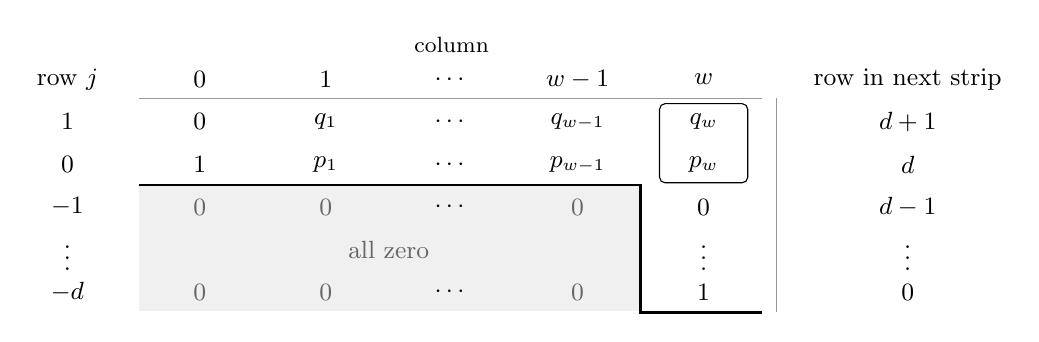
\begin{tikzpicture}[x=16mm,y=5.4mm,font=\small]
  \fill[black!6] (-.48,-3.45) rectangle (3.50,-.48);
  \draw[black!40] (-.48,1.56) -- (4.46,1.56);
  \draw[black!40] (4.58,-3.46) -- (4.58,1.56);
  \node at (-1.05,2) {row $j$};
  \node at (5.62,2) {row in next strip};
  \node[font=\footnotesize] at (2,2.82) {column};
  \foreach \k/\lbl in {0/0,1/1,2/{\cdots},3/{w-1},4/w}
    \node at (\k,2) {$\lbl$};
  \foreach \j/\old/\newrow in {1/1/{d+1},0/0/d,-1/{-1}/{d-1},-2/{\vdots}/{\vdots},-3/{-d}/0} {
    \node at (-1.05,\j) {$\old$};
    \node at (5.62,\j) {$\newrow$};
  }
  \node at (0,0) {$1$}; \node at (0,1) {$0$};
  \foreach \k/\lbl in {1/1,3/{w-1},4/w} {
    \node at (\k,0) {$p_{\lbl}$}; \node at (\k,1) {$q_{\lbl}$};
  }
  \foreach \j in {1,0,-1,-3} \node at (2,\j) {$\cdots$};
  \foreach \k in {0,1,3} {
    \node[text=black!60] at (\k,-1) {$0$};
    \node[text=black!60] at (\k,-3) {$0$};
  }
  \node[text=black!60] at (1.5,-2) {all zero};
  \node at (4,-1) {$0$}; \node at (4,-2) {$\vdots$}; \node at (4,-3) {$1$};
  \draw[line width=.9pt] (-.48,-.48) -- (3.50,-.48) -- (3.50,-3.48) -- (4.46,-3.48);
  \draw[rounded corners=2pt] (3.65,-.43) rectangle (4.35,1.43);
\end{tikzpicture}
\caption{A strip of width $w$ ending in a drop of depth $d$. The heavy line follows the bottom. At column $w$ the new binary word occupies old rows $-d,\ldots,-1$ and the boxed entries pass to rows $d,d+1$ of the next strip.}\label{fig:shared-column}
\end{figure}

\section{Differences between consecutive columns}\label{sec:diff}
Apply $\sigma$ entrywise to $B$ and write $B_\lambda=\sum_n\sigma(b_n)X^n$. In a fixed strip, write $V_{j,k}$ for its embedded cofactor entry at $(j,k)$. Encode rows zero through three as $V_k(y)=\sum_{j=0}^3 V_{j,k}y^j$, doing arithmetic modulo $y^4$. Set $S=1+y+y^2+y^3$. Lemma~\ref{lem:four} and the vanishing of row $-1$ give
\[
 (1+y)V_k+\lambda V_{k-1}=S \quad(1\le k\le w).
\]
Write $V_0=1+Hy^2+Gy^3$ and define $U,V$ by
\[
 ((1+y+\lambda)V_0-S)/\lambda=1+Uy^2+Vy^3\pmod{y^4}.
\]
For $k=1$, $(1+y)(V_1-V_0)=S-(1+y+\lambda)V_0$. Each subsequent difference is the previous one multiplied by $-\lambda/(1+y)$, by subtraction of consecutive recurrence equations. Hence
\begin{equation}\label{eq:diff}
 V_k-V_{k-1}=(-\lambda)^k(1+y)^{-k}(1+Uy^2+Vy^3)\pmod{y^4}.
\end{equation}
In particular all dependence on the previous strip is confined to $U,V$.

Let $p_v(\lambda),q_v(\lambda)$ be the sums in Lemma~\ref{lem:four} evaluated at $\lambda$ at the final step of the previous strip of width $v$. Its last column is the current strip's first. If the new drop has depth two, the word $10$ sits immediately below those two entries, so $H=p_v(\lambda)$ and $G=q_v(\lambda)$. These are the images under $\sigma$ of the boxed entries in Figure~\ref{fig:shared-column} with $w=v$. If the depth is three, the word is $100$, giving $H=0$, $G=p_v(\lambda)$. For a deeper drop, $H,G$ are adjacent digits in the new word and so form one of $(0,0),(1,0),(0,1)$. The finite sums satisfy
\[
 (1+\lambda)p_v(\lambda)=1+\lambda(-\lambda)^v,\qquad
 (1+\lambda)q_v(\lambda)+p_v(\lambda)-1=v(-\lambda)^{v+1}.
\]
Substitution in the definition of $U,V$ gives
\begin{equation}\label{eq:start}
 (U,V)=
 \begin{cases}
 ((-\lambda)^v,-v(-\lambda)^v),&d=2,\\
 (-1/\lambda,(-\lambda)^v),&d=3,\\
 (-1/\lambda,-1/\lambda),\ (1,0),\ \text{or }(-1/\lambda,1),&d\ge4.
 \end{cases}
\end{equation}
In every case $|U|\le R^v$ and $|V|\le vR^v$.

\section{A global bound for the column differences}\label{sec:filter}
At a fixed step $1\le k\le w$ of a strip, we use the binary product digits to bound a linear combination of the four differences $V_{j,k}-V_{j,k-1}$ in~\eqref{eq:diff}. The common factor $(1+y)^{-k}$ has alternating coefficients. In its product with $(1-y)^2$, each coefficient therefore has magnitude equal to the sum of the adjacent magnitudes with weights $1,2,1$. We apply this same second difference to the full polynomial in~\eqref{eq:diff}.

The other factor of the filter will control the global estimate. The endpoint terms in~\eqref{eq:array} act on rows by multiplication by $1+y$. Write $y=T^2$, so $1+y=TJ$, where $J=T+T^{-1}$ takes one step in either direction. After removing the shift $T$, the endpoint terms act by $J$ and the middle term shifts the column with coefficient $\lambda$. With a real variable $u$ in place of $J$, a homogeneous column solution satisfies $u h_s=-\lambda h_{s-1}$. It decays towards increasing column index $s$ for $|u|>R$ and towards decreasing $s$ for $|u|<R$. The estimate in Appendix~\ref{app:estimate} uses one derivative in $u$. Multiplying each geometric branch by $(u^2-R^2)^2$ makes its value and first derivative vanish at $|u|=R$, so it joins its zero extension with a continuous derivative. To obtain this double zero in row coordinates, take
\[
 Q(y)=(1+y)^2-R^2y,\qquad P(y)=(1-y)^2Q(y)^2.
\]
Indeed $Q(T^2)=T^2(J^2-R^2)$.

\begin{proposition}\label{prop:norm}
Let $0<r<m$ be integers, let $\lambda\in\mathbb C$ with $R=|\lambda|\ge1$, and let $B_\lambda\in\mathbb C[X]$. If $C=(1+X^m+\lambda X^r)B_\lambda$ is binary, then for every integer $N$,
\[
 \left|[X^N](1-X^r)P(X^m)B_\lambda(X)\right|<25R^3.
\]
\end{proposition}
Appendix~\ref{app:estimate} proves the proposition by counting walks on the integers. We apply it at the exponent of each of the three rows $j=1,2,3$.

Set $t=R^2-1\ge0$ and write $P_i=[y^i]P(y)$. In increasing powers of $y$ these coefficients are
\[
 1,\ -2t,\ t^2+2t,\ -2(1+t^2),\ t^2+2t,\ -2t,\ 1 .
\]
Let $N_0$ be the exponent of the cofactor entry at the local origin $(0,0)$. Then $(j,k)$ has exponent $N=N_0+jm+kr$. Write $\Delta V_{i,k}=V_{i,k}-V_{i,k-1}$ for every integer row $i$. Extracting the coefficient at $N$ gives the full row sum
\begin{equation}\label{eq:full-row}
 [X^N](1-X^r)P(X^m)B_\lambda(X)
    =\sum_{i=0}^6 P_i\,\Delta V_{j-i,k}
    =(-\lambda)^k f_{j,k}+E_{j,k},
\end{equation}
where
\[
 f_{j,k}=[y^j]P(y)(1+y)^{-k}(1+Uy^2+Vy^3).
\]
Indeed, $X^{im}$ selects row $j-i$ and $X^r$ shifts back one column. Equation~\eqref{eq:diff} accounts for the terms with $i\le j$. The remainder $E_{j,k}$ uses only negative rows.

For $k<w$ both columns vanish in negative rows, so $E_{j,k}=0$. For $k=w$, put $\eta_h=V_{h,w}$ for $h<0$. These are the digits of the new word, extended by zeros below its bottom. The embedding fixes those digits and $\eta_{-1}=0$ by Lemma~\ref{lem:geometry}. Since the preceding column vanishes there, the three remainders are
\[
\begin{aligned}
 E_{1,w}&=P_3\eta_{-2}+P_4\eta_{-3}+P_5\eta_{-4}+P_6\eta_{-5},\\
 E_{2,w}&=P_4\eta_{-2}+P_5\eta_{-3}+P_6\eta_{-4},\\
 E_{3,w}&=P_5\eta_{-2}+P_6\eta_{-3}.
\end{aligned}
\]
In the first row the positive coefficients sum to $(1+t)^2$ and the absolute values of the negative ones sum to $2(1+t^2)+2t\le 2(1+t)^2$. In the last two rows the positive coefficients sum to at most $(1+t)^2$ and the negative ones have total modulus $2t\le(1+t)^2$. Thus $|E_{1,k}|\le 2R^4$ and $|E_{2,k}|,|E_{3,k}|\le R^4$. By Proposition~\ref{prop:norm} and~\eqref{eq:full-row},
$R^k|f_{j,k}|\le 25R^3+|E_{j,k}|$. Using $R\ge1$ and dividing by $R^k$ gives
\begin{equation}\label{eq:constraint}
 |f_{1,k}|\le27R^{4-k},\qquad |f_{2,k}|,\ |f_{3,k}|\le26R^{4-k}.
\end{equation}

The three rows share a factor. Denote its quadratic and cubic coefficients by $B_k$ and $-L_k$, respectively.
\[
 P(y)(1+y)^{-k}=1-(k+2t)y+B_k y^2-L_k y^3\pmod{y^4}.
\]
At $k=0$ we read off $B_0=t^2+2t$, $L_0=2(1+t^2)$. Multiplication by $1+y$ takes step $k$ back to step $k-1$, so
\begin{equation}\label{eq:BL}
 B_k-B_{k-1}=k+2t,\qquad L_k-L_{k-1}=B_k .
\end{equation}
Multiplication by the initial factor $1+Uy^2+Vy^3$ recovers the three row differences in~\eqref{eq:constraint}.
\begin{equation}\label{eq:f}
 f_{1,k}=-(k+2t),\quad f_{2,k}=B_k+U,\quad
 f_{3,k}=-L_k-(k+2t)U+V .
\end{equation}

\section{Excluding a widest strip}\label{sec:short}
Take the final step $k$ of a widest strip. By~\eqref{eq:max}, $k\ge5$ and the preceding width is at most $k$. Thus $|U|\le R^k$ and $|V|\le kR^k$ by~\eqref{eq:start}. Divide~\eqref{eq:f} by $R^2=1+t$ and write
\[
 u=R^{k-2},\qquad z=26/u.
\]
With this scaling, $u$ bounds the inherited term $|U|/R^2$ and $z$ bounds the error from either of the last two rows. Equations~\eqref{eq:constraint} and~\eqref{eq:f} give
\begin{equation}\label{eq:three}
 \frac{k+2t}{1+t}\,u\le27,\qquad
 \frac{B_k}{1+t}\le u+z,\qquad
 \frac{L_k}{1+t}\le(2k+2t)u+z .
\end{equation}

It suffices to evaluate the lower bounds at width five. Summing~\eqref{eq:BL} gives
\[
 B_5=14(1+t)+(t-1)^2,\qquad
 L_5=(36+6t)(1+t)+(t-1)^2 .
\]
The sequence $B_k$ increases, and each subsequent increment of $L_k$ equals $B_k$. Hence
\begin{equation}\label{eq:growth}
 \frac{B_k}{1+t}\ge14,\qquad
 \frac{L_k}{1+t}\ge36+6t+14(k-5).
\end{equation}

We compare the last inequality of~\eqref{eq:three} with this growth, starting with the coefficient $2\cdot5=10$ of $u$. The first inequality of~\eqref{eq:three} gives $u<10$, since $(k+2t)/(1+t)=2+(k-2)/(1+t)\ge2+3/4$ by $R\le2$. The second gives $u+z\ge14$. As $uz=26$,
\[
 (10-u)(10-z)=126-10(u+z)<0 .
\]
Thus $z>10$ and $u=26/z<3$, while $u=R^{k-2}>1$. Since $(u-1)(z-10)>0$, we have $10u+z<uz+10=36$. The third inequality of~\eqref{eq:three} now gives
\[
 \frac{L_k}{1+t}\le (10u+z)+2(k-5+t)u
 <36+6(k-5+t),
\]
contradicting~\eqref{eq:growth} for every $k\ge5$. This excludes a fractional $a$. The induction following~\eqref{eq:basic} finishes the proof of Theorem~\ref{thm:main}.

\appendix
\section{A coefficient estimate from walks on the integers}\label{app:estimate}
We prove Proposition~\ref{prop:norm}. Its left side involves the unknown cofactor. We will express it as a weighted sum of differences of the known product digits and bound the sum of the absolute weights.

\subsection{Two identities for polynomial coefficients}
Write $J=T+T^{-1}$. For a real polynomial $f$ let $b_d(f)=[T^d]f(J)$ and $L(f)=b_0(f)$. Each factor of $J$ takes a step of size $1$ or $-1$, so counting returns to the origin gives
\begin{equation}\label{eq:walk-moments}
 L(u^{2n})=\binom{2n}{n},\qquad L(u^{2n+1})=0 .
\end{equation}
For a real Laurent polynomial $H$ write $H^*(T)=H(T^{-1})$. The constant term of $HH^*$ is the sum of the squares of the coefficients of $H$. Apply this first to $f(J)$ and then to $T\,d(f(J))/dT=(T-T^{-1})f'(J)$. Since $(T-T^{-1})(T-T^{-1})^*=4-J^2$, we obtain
\begin{equation}\label{eq:walk-energy}
 \sum_d b_d(f)^2=L(f^2),\qquad
 \sum_d d^2 b_d(f)^2=L\big((4-u^2)f'(u)^2\big).
\end{equation}

To extend~\eqref{eq:walk-energy} to the column functions we first bound $L$ in the uniform norm. The functional $L$ is positive on polynomials nonnegative on $[-2,2]$. Indeed, factor such a polynomial over the reals. Interior roots occur to even order, conjugate pairs give sums of two squares, and the remaining linear factors can be written $c\pm u$ with $c\ge2$, up to an overall positive constant. After substitution,
\[
 c\pm J=(c-2)+(1\pm T)(1\pm T^{-1}).
\]
Products of sums of terms $HH^*$ again have this form, so their constant term is nonnegative. Applying positivity to $\|f\|_\infty\pm f$ gives $|L(f)|\le\|f\|_\infty$. By Weierstrass approximation, $L$ extends uniquely to a positive functional on $C[-2,2]$.

For $f\in C^1[-2,2]$, approximate $f'$ uniformly by polynomials and integrate them from zero, matching $f(0)$. The resulting polynomials converge to $f$ in $C^1$. Applying both identities in~\eqref{eq:walk-energy} to differences of approximants shows that the coefficient vectors are Cauchy in the norm $(\sum_d(1+d^2)|b_d|^2)^{1/2}$. The same argument for two choices of approximants gives the same limit, which defines $b_d(f)$. Passing to the limit gives both energy identities. If $p_n\to f$ in $C^1$, then $up_n\to uf$ there as well. The polynomial shift identity therefore gives
\begin{equation}\label{eq:walk-shift}
 b_d(uf)=b_{d-1}(f)+b_{d+1}(f).
\end{equation}

\subsection{Solving the column recurrence}
Put $x=R^2$ and $w(u)=4-u^2$. Since $(1-T^2)^2=-T^2w(J)$ and $Q(T^2)=T^2(J^2-x)$, the filter is $P(T^2)=-T^6p(J)$ with $p(u)=w(u)(u^2-x)^2$. We therefore seek scalar functions $f_s$, $s\in\Z$, satisfying
\begin{equation}\label{eq:walk-scalar}
 u f_s+R f_{s-1}=\mathbf 1_{s=0}\,p .
\end{equation}
For $j\ge0$ the decaying geometric solutions on the two sides of $|u|=R$ are
\[
 f_j(u)=p(u)\frac{(-R)^j}{u^{j+1}}\quad(|u|>R),\qquad
 f_{-j-1}(u)=p(u)\frac{(-u)^j}{R^{j+1}}\quad(|u|<R).
\]
Each function is zero outside its indicated region. The factor $(u^2-x)^2$ makes both extensions $C^1$, including at $|u|=R$, and substitution verifies~\eqref{eq:walk-scalar}.

Set $k_{d,s}=b_d(f_s)$. By~\eqref{eq:walk-shift}, multiplying the array $\sum_{d,s}k_{d,s}T^d Z^s$ by $J+RZ$ gives $p(J)$ coefficient by coefficient. We will prove
\begin{equation}\label{eq:walk-norm}
 \sum_{d,s}|k_{d,s}|<25R^3.
\end{equation}
Assuming~\eqref{eq:walk-norm}, substitute $T=X^m$ and $Z=(\lambda/R)X^{2r-m}$. The coefficient of $X^n$ in the resulting bilateral series $K$ is
\[
 K_n=\sum_{md+(2r-m)s=n} k_{d,s}(\lambda/R)^s .
\]
These fibers partition $\Z^2$ and $|\lambda/R|=1$, so each sum converges absolutely and $\sum_n|K_n|\le\sum_{d,s}|k_{d,s}|$. A monomial in $T,Z$ translates the indices and multiplies by a constant phase. Hence grouping by these fibers commutes with multiplication by any finite Laurent polynomial, including $J+RZ$. Under this substitution $T(J+RZ)=1+X^{2m}+\lambda X^{2r}$. Using the formulas for $P(T^2)$ and $C$, the array identity gives
\[
 (1-X^{2r})P(X^{2m})B_\lambda(X^2)
       =-X^{5m}K(X)(1-X^{2r})C(X^2).
\]
Every coefficient of $(1-X^{2r})C(X^2)$ is a difference of two binary digits and has modulus at most one. At exponent $2N$ the right side is therefore bounded in modulus by $\sum_n|K_n|$. The left side is the coefficient at $N$ in Proposition~\ref{prop:norm}.

\subsection{Bounding the absolute sum}
Pair the columns $s=j$ and $s=-j-1$, $j\ge0$. Since $p(u)$ is even, their functions have signs $(-1)^{j+1}$ and $(-1)^j$, respectively, under $u\mapsto -u$. Also $J(-T)=-J(T)$ gives $b_d(f(-\,\cdot))=(-1)^d b_d(f)$, first for polynomials and then by approximation. Consequently
\[
 k_{d,j}=0\ \text{unless }d\equiv j+1\pmod 2,\qquad
 k_{d,-j-1}=0\ \text{unless }d\equiv j\pmod 2 .
\]
For each $(j,d)$ at most one coefficient contributes. With $\ell=j+1/2$, give it weight $\omega=\ell(\ell^2+9+d^2)$. Applying Cauchy--Schwarz on finite rectangles of $(j,d)$ and then increasing the rectangles bounds the square of the left side of~\eqref{eq:walk-norm} by $SE$, where
\[
 S=\sum_{j\ge0,\ d\in\Z}\frac1{\ell(\ell^2+9+d^2)},\qquad
 E=\sum_{j\ge0,\ d\in\Z}\omega\bigl(|k_{d,j}|^2+|k_{d,-j-1}|^2\bigr).
\]
For $b^2=\ell^2+9-1/12$, the mean of $b^2+t^2$ on $[d-1/2,d+1/2]$ is $\ell^2+9+d^2$. Convexity of the reciprocal gives $\sum_d(\ell^2+9+d^2)^{-1}\le\int_{\mathbb R}(b^2+t^2)^{-1}dt=\pi/b$. Since $b\ge\max(3,\ell)$,
\[
 S/\pi\le \tfrac13(2+2/3)+\sum_{j\ge2}(j+1/2)^{-2}
 \le\tfrac89+\tfrac12=\tfrac{25}{18},
\]
where $(j+1/2)^{-2}\le 1/j-1/(j+1)$.

It remains to compute $E$ by~\eqref{eq:walk-energy}. For fixed $u$ with $|u|\ne R$, write $w g_j$ for the active function in the pair $f_j,f_{-j-1}$, with $g_j$ given by the same formula with $p$ replaced by $(u^2-x)^2$. Write $h=u^2$ and $M(h)=(h+x)(h-x)^2/2$. The three scalar sums needed are
\begin{equation}\label{eq:walk-sums}
 \sum_j\ell g_j^2=M(h),\qquad
 \sum_j\ell^3 g_j^2=M(h)/4+3hx(h+x),\qquad
 \sum_j\ell (g_j')^2=\tfrac32(3h^2+x^2).
\end{equation}
For the first two, put $q=\min(h,x)/\max(h,x)$. Then $g_j^2=\max(h,x)^3(1-q)^4q^j$. The geometric sum gives $\sum\ell q^j=(1+q)/(2(1-q)^2)$ and $\sum(\ell^3-\ell/4)q^j=3q(1+q)/(1-q)^4$. For the derivative sum take $v$ near $u$ in the same region. Summing the geometric products on either side gives the same expression
\[
 \sum_j\ell g_j(u)g_j(v)=
 \frac{uv+x}{2}\frac{(u^2-x)^2(v^2-x)^2}{(uv-x)^2}.
\]
Writing $(u^2-x)(v^2-x)=(uv-x)^2-x(u-v)^2$ turns this expression into
\[
 M(uv)-x(uv+x)(u-v)^2+
 \frac{x^2(uv+x)(u-v)^4}{2(uv-x)^2}.
\]
Since $u^2\ne x$, the last term has zero mixed derivative at $v=u$. The mixed derivative of the first two terms there is $(hM'(h))'+2x(h+x)=\tfrac32(3h^2+x^2)$, as asserted. On a sufficiently small closed neighborhood of $(u,u)$ the geometric ratio has modulus at most $\rho<1$. The terms and their first and mixed derivatives are bounded there, for $j\ge2$, by a constant times $(j+1)^3\rho^{j-2}$. This summable majorant justifies termwise differentiation.

For each finite set of column indices,~\eqref{eq:walk-energy} expresses its contribution to $E$ as $L$ applied to the corresponding sum of $\ell\big((\ell^2+9)f_s^2+w(f_s')^2\big)$. These summands are nonnegative. Away from $|u|=R$ the cross term in $(w g_j)'^2$ uses $\sum_j\ell g_jg_j'=uM'(h)$, obtained by differentiating the first identity in~\eqref{eq:walk-sums}. Substituting all three sums gives the polynomial
\[
 D(h)= w^2\big(\tfrac{37}{4}M(h)+3hx(h+x)\big)
       +\tfrac32 w^3(3h^2+x^2)+4hw M(h)-4hw^2M'(h),
 \qquad w=4-h .
\]
At a switching point $h=x$ in the interval, every $f_s$ and $f_s'$ vanishes. The polynomial takes the value
\[
 D(x)=6x^3(4-x)^2+6x^2(4-x)^3=24x^2(4-x)^2,
\]
which is positive for $1\le x<4$ and zero at $x=4$. Thus for $R<2$ the equality for the full density holds only off the switching points. For a finite set of columns $F$, let $H_F(u)$ be its sum of the continuous energy densities above. On $|u|\ne R$, nonnegativity gives $H_F(u)\le D(u^2)$. Continuity extends this inequality to the whole interval. Applying the positive functional $L$ to this finite sum and then taking the supremum over $F$ gives $E\le L(D(u^2))$.

The polynomial $D$ has degree five in $h$. By~\eqref{eq:walk-moments}, substituting $h=u^2$ pairs its coefficients, in ascending order, with the return counts $1,2,6,20,70,252$. This gives
\[
 L(D(u^2))=\tfrac14(127x^3+94x^2-23x+374)\le143x^3
 \qquad(x\ge1).
\]
Indeed $374-23x\le351$ for $x\ge1$. Finally $143\pi<450$ by $\pi<22/7$, so $SE\le(25\pi/18)143R^6<625R^6$. This proves~\eqref{eq:walk-norm} and Proposition~\ref{prop:norm}.

\medskip
\noindent\textit{Verification.} The supplementary script \texttt{check-walk-energy.py} reproduces the scalar identities and the moment evaluation in exact arithmetic. The accompanying Lean formalization proves Theorem~\ref{thm:main}, including Proposition~\ref{prop:norm}, using mathlib.

\begin{thebibliography}{1}
\bibitem{dvorsky}
A. Dvorsky, \emph{The unfair 0--1 polynomial problem and high-degree trinomials}, 2026, \href{https://arxiv.org/abs/2608.19173v2}{arXiv:2608.19173v2}.
\bibitem{dvorsky-finite}
A. Dvorsky, \emph{Trinomials of the type $1+ax^2+x^k$ in the unfair $0$--$1$ polynomial problem}, manuscript, version~4, 4 August 2026.
\bibitem{ghidelli}
L. Ghidelli, \emph{Progress on the unfair 0--1-polynomials conjecture using linear recurrences and numerical analysis}, 2022, \href{https://arxiv.org/abs/2209.09843}{arXiv:2209.09843}.
\bibitem{hare}
K. G. Hare, \emph{Computational progress on the unfair 0--1 polynomial conjecture}, Experimental Mathematics, published online 15 July 2025, \href{https://doi.org/10.1080/10586458.2025.2527786}{doi:10.1080/10586458.2025.2527786}.
\bibitem{hasanbegovic}
E. Hasanbegovi\'c, \emph{Structural results on the unfair 0--1 polynomial conjecture}, 2026, \href{https://arxiv.org/abs/2611.14596}{arXiv:2611.14596}.
\end{thebibliography}
\end{document}
